\documentclass{article}

% package
\usepackage[margin=.5in]{geometry}
\usepackage{xcolor}
\usepackage{float}
\usepackage{tikz}
\usepackage{enumitem}
\usepackage{amsmath,amssymb}
\usepackage{pgffor}

% presets
\pagecolor{black}
\color{white}
\usetikzlibrary{
	arrows.meta,
	automata,
	positioning
}
\tikzset{
	node distance=1in,
	every loop/.append style={
		-Straight Barb
	},
	every initial by arrow/.style={
		-Straight Barb
	},
	every edge/.append style={
		-Straight Barb
	},
	initial text=,
	double=black
}

% macro
\def \answer {\item [$\rightarrow$]}
\def \RE {Regular Expression~}
\def \RL {Regular Language~}
\def \FA {Finite Automata~}

\newcommand{\indentpar}[2]{
	\begin{itemize}[leftmargin=#1,label=]
		\item #2
	\end{itemize}
}

\begin{document}
	\begin{enumerate}[label=\arabic*)]
		\item Define Regular expression ? Obtain a Regular Expression for the language
		\begin{enumerate}[label=\alph*)]
			\item $\text{L} = \{a^{2n}\ b^{2m}~|~n \ge 0,~m \ge 0\}$
			\item $\text{L} = \{\text{W}~|~\text{W} \in \{0,1\} \ast
				\text{ with at least three consecutive zeros}\}$
			\item $\text{L} = \{\text{W} : \text{N}_a(\text{W}) \mod 3=0
				\text{, where } \text{W} \in (a,b) \ast\}$
			\item $\text{L} = \{a^n\ b^m~|~m+n \text{ is even}\}$
			\item $\text{L} = \{a^n\ b^m~|~m \ge 1,~n \ge 1,~nm \ge 3\}$
			\item To accept strings of $a$'s and $b$'s such that every block of four consecutive symbols
				contain at least two $a$'s
		\end{enumerate}
		\answer A regular expression is a recursively defined as follows
			\begin{enumerate}[label=\roman*)]
				\item $\varnothing$ is a \RE denoting an empty language
				\item $\varepsilon$ is a \RE indicates the language containing an empty string
				\item $a$ is a \RE which indicates the language containing only $\{a\}$
				\item If R is a \RE denoting the language $\text{L}_\text{R}$ and S is a \RE denoting the
					language $\text{L}_\text{S}$, then
					\begin{enumerate}[label=\alph*)]
						\item $\text{R}+\text{S}$ is a \RE corresponding to the language
							$\text{L}_\text{R} \cup \text{L}_\text{S}$
						\item $\text{R}\cdot\text{S}$ is a \RE corresponding to the language
							$\text{L}_\text{R} \cap \text{L}_\text{S}$
					\end{enumerate}
				\item The expression obtained by applying any of the rules from 1 to 4 are regular expressions
			\end{enumerate}
			Regular expressions for following languages are
			\begin{enumerate}[label=\alph*)]
				\item $\text{L} = \{a^{2n}\ b^{2m}~|~n \ge 0,~m \ge 0\}$ \\
					$((a+b)(a+b))\ast$ OR $(a+b)^2\ast$
				\item $\text{L} = \{\text{W}~|~\text{W} \in \{0,1\} \ast
					\text{ with at least three consecutive zeros}\}$ \\
					$(0+1)\ast000(0+1)\ast$
				\item $\text{L} = \{\text{W} : \text{N}_a(\text{W}) \mod 3=0
					\text{, where } \text{W} \in (a,b) \ast\}$ \\
					$(aaa+b)\ast$ OR $(a^3+b)\ast$
				\item $\text{L} = \{a^n\ b^m~|~m+n \text{ is even}\}$ \\
					$(a(aa)\ast b(bb)\ast+(aa)\ast(bb)\ast)$
				\item $\text{L} = \{a^n\ b^m~|~m \ge 1,~n \ge 1,~nm \ge 3\}$ \\
					$(aaa)a\ast bb\ast+(bbb)b\ast aa\ast$ OR $(aaab+bbba)a\ast b\ast$ OR $(aaab+bbba)(a+b)\ast$
				\item To accept strings of $a$'s and $b$'s such that every block of four consecutive symbols
					contain at least two $a$'s \\
					$~~aa(a+b)(a+b)+a(a+b)a(a+b)+a(a+b)(a+b)a+(a+b)a(a+b)a+(a+b)(a+b)aa \\
					(aa(a+b)(a+b)+a(a+b)a(a+b)+a(a+b)(a+b)a+(a+b)a(a+b)a+(a+b)(a+b)aa)*$
						$$\text{OR}$$
					$~a^2(a+b)^2+(a(a+b))^2+a(a+b)^2a+((a+b)a)^2+(a+b)^2a^2 \\
					(a^2(a+b)^2+(a(a+b))^2+a(a+b)^2a+((a+b)a)^2+(a+b)^2a^2)*$
			\end{enumerate} \newpage
		
		\item State and Prove Pumping lemma for \RL 
		\begin{enumerate}[label=\roman*)]
			\item Show that language $\text{L}= \{\text{W}\text{W}^\text{R}~|~n \ge 0\}$ is not regular
			\item show that language $\text{L}= \{a^n\ b^n~|~n \ge 0\}$ is not regular
		\end{enumerate}
		\answer \textbf{Theorem}
			\begin{itemize}
				\item Let $\text{M}=(\text{Q},\sum,\delta,q_0,\text{F})$ be an \FA and has $n$ number of states
				\item Let L be the \RL accepted by M
				\item $\forall$ string $x$ in L, $\exists$ a constant $n$ such that $|x|\ge n$
				\item If the string $x$ is broken into three substrings $u$, $v$ and $w$ such that $x=uvw$
				\item Where,
				\begin{itemize}
					\item $v\ne\varepsilon$ ~~i.e. $|v|\ge1$
					\item $|uv|\le n$
				\end{itemize}
				\item Implies $uv^iw\in \text{L}$ where, $i\ge0$
			\end{itemize}

		\textbf{Proof}
			\begin{itemize}
				\item Let $\text{M}=(\text{Q},\sum,\delta,q_0,\text{F})$ be an \FA and $n$ be number of states
				\item Let L is the language accepted by DFA and is regular
				\item Let $x=a_1a_2a_3\cdots a_m$ where, $m\ge n$ and $\forall a_i \in \sum$
				\item Since we have $m$ input the total $m+1$ states are $q_0,q_1,\cdots,q_m$ where, $q_0$ and
					$q_m$ are initial and final state respecitvely.
					\begin{figure}[H]
						\centering
						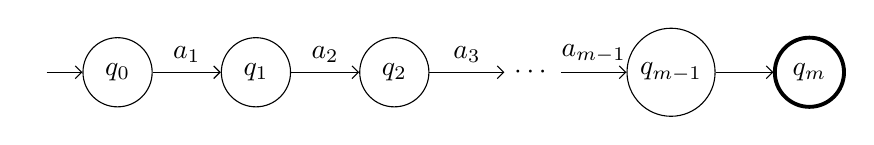
\begin{tikzpicture}[node distance=5em]
							\draw
								node [initial,state]                (q0)   {$q_0$}
								node [state,right of=q0]            (q1)   {$q_1$}
								node [state,right of=q1]            (q2)   {$q_2$}
								node [right of=q2]                  (dots) {$\cdots$}
								node [state,right of=dots]          (qm1)  {$q_{m-1}$}
								node [state,accepting,right of=qm1] (qm)   {$q_m$}

								(q0)   edge[above] node {$a_1$}     (q1)
								(q1)   edge[above] node {$a_2$}     (q2)
								(q2)   edge[above] node {$a_3$}     (dots)
								(dots) edge[above] node {$a_{m-1}$} (qm1)
								(qm1)  edge                         (qm)
							;
						\end{tikzpicture}
					\end{figure}
				\item Since $|x|\ge n$, by the pegion hole principle it is not possible to have distinct
					transitions one of the state can have a loop
				\item Let the string $x$ is divided into three substrings as shown below
					\begin{itemize}
						\item The first group is the prefix string ~i.e. $u=a_1a_2\cdots a_i$
						\item The second group is the loop string i.e. $v=a_{i+1}a_{i+2}\cdots a_{j-1}a_j$
						\item The third group is the suffix string ~i.e. $w=a_{j+1}a_{j+2}\cdots a_m$
					\end{itemize}
					\begin{figure}[H]
						\centering
						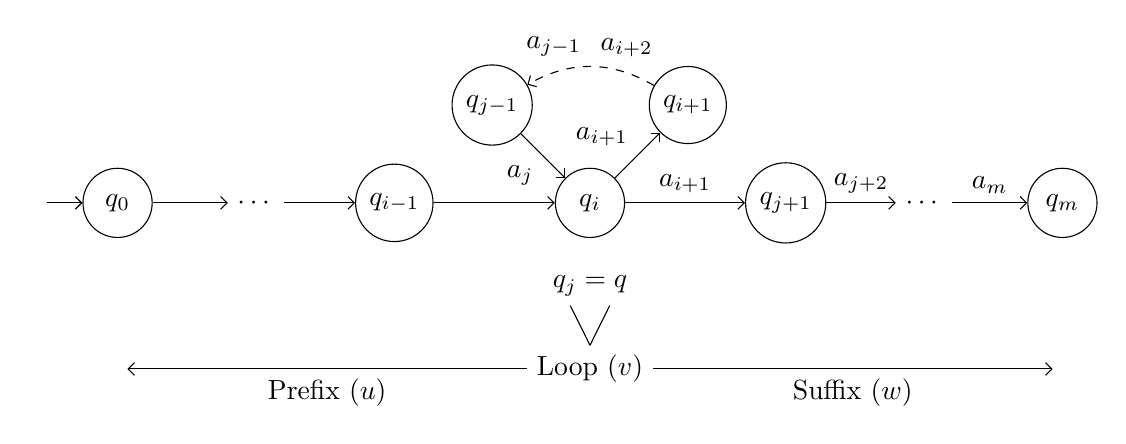
\begin{tikzpicture}[node distance=5em]
							\draw
								node [initial,state]            (q0)  {$q_0$}
								node [right of=q0]              (d0)  {$\cdots$}
								node [state,right of=d0]        (qi1) {$q_{i-1}$}
								node [state,above right of=qi1] (qj1) {$q_{j-1}$}
								node [state,below right of=qj1] (qi)  {$q_i$}
								node [state,above right of=qi]  (q1i) {$q_{i+1}$}
								node [state,below right of=q1i] (q1j) {$q_{j+1}$}
								node [right of=q1j]             (d1)  {$\cdots$}
								node [state,right of=d1]        (qm)  {$q_m$}

								node [node distance=3em,below of=qi] (qj) {$q_j=q$}
								node [node distance=3em,below of=qj] (v)  {Loop $(v)$}
								node [node distance=6em,below of=q0] (u)  {}
								node [node distance=6em,below of=qm] (w)  {}

								(q0)  edge                                (d0)
								(d0)  edge                                (qi1)
								(qi1) edge                                (qi)
								(qi)  edge [above]       node {$a_{i+1}$} (q1j)
								(q1j) edge [above]       node {$a_{j+2}$} (d1)
								(d1)  edge [above]       node {$a_m$}     (qm)
								(qj1) edge [below left]  node {$a_j$}     (qi)
								(qi)  edge [above left]  node {$a_{i+1}$} (q1i)
								(q1i) edge [dashed,bend right]
									node [above right] {$a_{i+2}$}
									node [above left]  {$a_{j-1}$}        (qj1)

								(qj.315) -- (v.90)
								(qj.225) -- (v.90)

								(v) edge [below] node {Prefix $(u)$} (u)
								(v) edge [below] node {Suffix $(w)$} (w)
							;
						\end{tikzpicture}
					\end{figure}
				\item Prefix string $u$ takes the machine from $q_0$ to $q_i$ \\
					Loop string $v$ takes the machine from $q_i$ to $q_i$ \\
					Suffix string $v$ takes the machine from $q_i$ to $q_m$
				\item When $i=0$, the minimum string accepted by FA is $uw$ \\
					$~~\forall~~i>0$ strings the loop string is looped over $q_i$ to $q_i$, then goes to
					later states, and final state
			\end{itemize} \newpage

		\item Obtain an $\varepsilon$NFA for the following regular expressions
		\begin{enumerate}[label=\roman*)]
			\item $aa(a+b) \ast$
			\item $a \ast+b \ast+c \ast$
			\item $0 + 01 \ast$
		\end{enumerate}
		
		\item Obtain a regular expression for the FA Shown below
		\begin{figure}[H]
			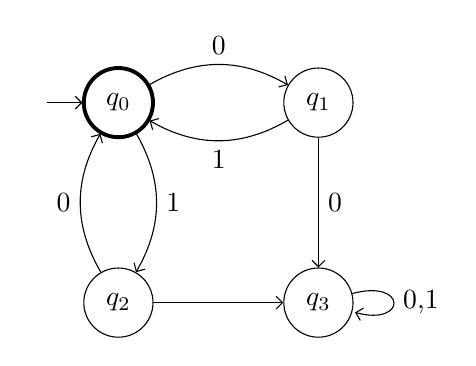
\begin{tikzpicture}
				\draw
					node [state,initial,accepting] (q0) {$q_0$}
					node [state,right of=q0]       (q1) {$q_1$}
					node [state,below of=q0]       (q2) {$q_2$}
					node [state,right of=q2]       (q3) {$q_3$}
	
					(q0) edge [bend left,above]  node {0}   (q1)
					(q1) edge [bend left,below]  node {1}   (q0)
					(q2) edge [bend left,left]   node {0}   (q0)
					(q0) edge [bend left,right] node {1}   (q2)
					(q2) edge                               (q3)
					(q1) edge [right]            node {0}   (q3)
					(q3) edge [loop right]       node {0,1} (q3)
				;
			\end{tikzpicture}
		\end{figure}
		
		\item Show that Regular Languages are Closed under Complement and Intersections with an example
	
		\item Define Context Free Grammar. Design CFG for the following Languages
		\begin{enumerate}[label=\roman*)]
			\item $\text{L} = \{0^m\ 1^m\ 2^n~|~m \ge 1,~n \ge 0\}$
			\item $\text{L} = \{a^n\ b^m~|~n \ge 0, m>n\}$
			\item $\text{L} = \{a^n\ b^m\ c^k~|~n+2m=k ~~~\forall~n \ge 0,~m \ge 0\}$
			\item $\text{L} = \{\text{W}~|~\text{N}_a(\text{W})=\text{N}_b(\text{W})\}$
		\end{enumerate}
	
		\item Obtain the Left Most Derivation, Right Most Derivation and Parse Trees for the string
			``$\text{I}_d+\text{I}_d \ast \text{I}_d$" using the grammar
			$\text{E} \to \text{E}+\text{E}~|~\text{E} \ast \text{E}~|~\text{E}-\text{E}~|~\text{E}/\text{E}~|~
				\text{E} ^\wedge \text{E}~|~\text{I}_d$
	
		\item Obtain the Left Most Derivation, Right Most Derivation and Parse Trees for the string ``$aaabab$"
			using the grammar
			\begin{itemize}[label=]
				\item $\text{S} \to \text{A}b\text{B}$
				\item $\text{S} \to \text{A}a~|~\varepsilon$
				\item $\text{S} \to \text{A}b~|~\text{B}b~|~\varepsilon$
				\item $\text{S} \to a~|~\varepsilon$
			\end{itemize}
	
		\item Define PDA ?
		\begin{enumerate}[label=\roman*)]
			\item Design PDA to accept the language by final state method. \\
				$\text{L(M)} = \{\text{W}~|~\text{W} \in (a+b) \ast \text{ and } \text{N}_a(\text{W}) = 
				\text{N}_b(\text{W})\}$, where number of $a$'s in string W is equal to number of \\ $b$'s in W
			\item Draw the transition diagram and write the sequence of moves made by PDA to accept the string
				``$aababb$''
		\end{enumerate}
	
		\item Define PDA ?
		\begin{enumerate}[label=\roman*)]
			\item Design PDA to accept the language by final state method. \\
				$\text{L(M)} = \{\text{WC}\text{W}^\text{R} \text{, where W } \in (a+b) \ast \}$, where
				$\text{W}^\text{R}$ is the reverse of W
			\item Draw the transition diagram and write the sequence of moves made by PDA to accept the string
				``$aab\text{C}baa$"
		\end{enumerate}
	
		\item Define Ambiguity.
			\begin{itemize}
				\item [i)] Consider the grammar
					$\text{E} \to \text{E}+\text{E}~|~\text{E} \ast \text{E}~|~\text{E}~|~\text{I}_d$. \\
					Find the Left most derivation, Right most derivation and Parse Trees for the string
					$\text{\text{I}}_d+\text{I}_d \ast \text{I}_d$ and show that grammar is ambiguous
			\end{itemize}
	
		\item Let $\sum = \{a,b\}$, Obtain a grammar G Generating set of all palindromes over $\sum$
	
		\item What is the language generated by the grammar
			\begin{align*}
				& \to \text{OA}~|~\varepsilon \\
				\text{A} & \to 1\text{S}
			\end{align*}
	\end{enumerate}
\end{document}
